%%%%%%%%%%%%%%%%%%%%%%%%%%%%%%%%%%%%%%%%%%%%%%%%%%%%%%%%%%%%%%%%%%%%%%%%%%%%%%%%%%%%%%%%%%%%%%%%%%%%%%%%%%%%%%%%%%%%
%%%%%%%%%%%%%%%%%%%%%%%%%%%%%%%%%%%%%%%%%%%%%%%%%%%%%%%%%%%%%%%%%%%%%%%%%%%%%%%%%%%%%%%%%%%%%%%%%%%%%%%%%%%%%%%%%%%%
%%% ARTÍCULO
%%%%%%%%%%%%%%%%%%%%%%%%%%%%%%%%%%%%%%%%%%%%%%%%%%%%%%%%%%%%%%%%%%%%%%%%%%%%%%%%%%%%%%%%%%%%%%%%%%%%%%%%%%%%%%%%%%%%
%%%%%%%%%%%%%%%%%%%%%%%%%%%%%%%%%%%%%%%%%%%%%%%%%%%%%%%%%%%%%%%%%%%%%%%%%%%%%%%%%%%%%%%%%%%%%%%%%%%%%%%%%%%%%%%%%%%%
%\clearpage % Se recomienda dejar solo los datos del resumen en la primera página, sin embargo, esto no es obligatorio.

\section{Introducción}

Este texto de instrucciones modelo ha sido elaborado para que los autores puedan presentar los artículos de forma estandarizada.
%
Se ha adaptado del modelo de la \href{https://revista.acustica.org.br}{Revista Acústica y Vibraciones}, siendo de uso para el XIII~Congreso Iberoamericano de Acústica (FIA 2024).
Esto proporcionará una uniformidad en el formateo de los artículos completos del evento.
En este modelo se presentan las principales directrices para la elaboración del artículo completo en lo que respecta a la presentación de contenido, gráfica, estructura, diagramación y al procedimiento para la presentación de los artículos.
%
Este documento ya cuenta con el formateo de estilos personalizados para la elaboración del artículo. El autor puede, por lo tanto, utilizar este archivo como modelo para esa finalidad. Se pondrán a disposición modelos (\textit{templates}) en Microsoft Word (\texttt{.docx}) y \LaTeX\xspace (\texttt{.tex}). Esta versión también está disponible en \href{https://www.overleaf.com/read/tjbcfwbtfdtz\#869489}{Overleaf} y en \href{https://github.com/willdfonseca/latex}{GitHub} --- siendo aún compatible con Windows, Mac y Linux.
Los autores son responsables del contenido, elaboración y envío de los artículos de acuerdo con el presente modelo.

El texto completo deberá estar en interlineado simple, tipografía Times New Roman tamaño 12~pt y párrafo con espaciado de 0~pt antes y 6~pt después. Es práctica común la escritura de artículos científicos en impersonal, por lo tanto, esto es recomendable. Además, se aceptarán en lengua culta\footnote{Haga uso de correctores ortográficos y/o de gramática, tanto Ms Word como Overleaf los poseen, se indica además el uso de otras herramientas como el \href{https://languagetool.org/es}{Language Tool}.} portuguesa, inglesa\footnote{Artículos en lengua extranjera escritos por no nativos deben, preferentemente, recibir revisión profesional.} y española\footnotemark[2].


%%%%%%%%%%%%%%%%%%%%%%%%%%%%%%%%%%%%%%%%%%%%%%%%%%%%%%%%%%%%%%%%%%%%%%%%%%%%%%%%%%%%%%%%%%%%%%%%%%%%%%%%%%%%%%%%%%%
%%%%%%%%%%%%%%%%%%%%%%%%%%%%%%%%%%%%%%%%%%%%%%%%%%%%%%%%%%%%%%%%%%%%%%%%%%%%%%%%%%%%%%%%%%%%%%%%%%%%%%%%%%%%%%%%%%%
\section{Orientaciones básicas}

En esta sección hay un resumen de cómo debe construirse el artículo. Para más detalles, consulte las secciones subsecuentes.

\vspace{-8pt}
\begin{enumerate} \itemsep=2pt
    \item Los modelos en LaTeX y Word proporcionados ya contienen todas las configuraciones descritas en este documento. Además, este manuscrito proporciona simultáneamente instrucciones para las dos plataformas de diagramación de texto.
	\item La primera página debe contener (para las lenguas portuguesa y española) título, autores, afiliaciones, resumen, palabras clave, \textit{title}, \textit{abstract} y \textit{keywords}. Las presentaciones en inglés pueden contener solo autores, afiliaciones, \textit{title}, \textit{abstract} y \textit{keywords} (sin versiones en portugués o español).
	\item El texto debe estar escrito en lengua culta vigente.
	\item El número de páginas debe ser como mínimo 6 y como máximo 15, contando desde la página que contiene el título, hasta el final de las referencias (incluyendo apéndices, si los hay).
	\item El tamaño del papel es A4, con márgenes: superior de 2,0~cm, inferior de 2,0~cm, izquierda de 1,8~cm y derecha de 1,8~cm (el espaciado entre columnas es de 1,0~cm).
	\item El texto debe estar escrito con tipografía Times New Roman con tamaño 12~pt (conforme a este modelo).
	\item El artículo puede contener figuras, tablas, cuadros, códigos y ecuaciones. En el texto, si es necesario, se pueden colocar enlaces. También se aceptan animaciones, siempre y cuando estén diagramadas como figuras.
	\item Se entiende que un artículo técnico tenga una estructura lógica, descriptiva y contenido susceptible de reproducción, concluyendo en las referencias del trabajo.
\end{enumerate}


%%%%%%%%%%%%%%%%%%%%%%%%%%%%%%%%%%%%%%%%%%%%%%%%%%%%%%%%%%%%%%%%%%%%%%%%%%%%%%%%%%%%%%%%%%%%%%%%%%%%%%%%%%%%%%%%%%%
%%%%%%%%%%%%%%%%%%%%%%%%%%%%%%%%%%%%%%%%%%%%%%%%%%%%%%%%%%%%%%%%%%%%%%%%%%%%%%%%%%%%%%%%%%%%%%%%%%%%%%%%%%%%%%%%%%%
\section{Documento y presentación}

Siempre coloque texto en secciones y subsecciones, no las deje huérfanas (abriendo una sección y pasando directamente a la subsección).

%%%%%%%%%%%%%%%%%%%%%%%%%%%%%%%%%%%%%%%%%%%%%%%%%%%%%%%%%%%%%%%%%%%%%%%%%%%%%%%%%%%%%%%%%%%%%%%%%%%%%%%%%%%%%%%%%%%
\subsection{Primera página}

La primera página debe contener los siguientes elementos colocados por los autores: título, autores, afiliaciones, resumen, palabras clave, \textit{title}, \textit{abstract} y \textit{keywords}.
%
En caso de que el título completo sea muy extenso, se solicita una versión corta para que sea incluida en el encabezado de las páginas del artículo.

El resumen del artículo podrá tener entre 150 y 200 palabras (en tipografía de 11~pt). El resumen, las palabras clave, \textit{title}, \textit{abstract} y \textit{keywords} constituyen la primera página del artículo; se recomienda no extenderse a la segunda página.
Debe hacer una presentación concisa del artículo técnico-científico, conteniendo una introducción, el objetivo, una síntesis de la metodología, el principal resultado y la principal conclusión (preferiblemente en ese orden). No es necesario separar en ítems o secciones dentro del resumen. Así, el lector puede conocer la esencia del trabajo. Recuerde que el resumen es como el \textit{tráiler} de una película; las personas estarán interesadas en leer completamente el artículo si el resumen les interesa. El resumen no debe contener información nueva no incluida en el artículo; abreviaturas indefinidas; discusión previa de otra literatura; referencias y citas y exceso de detalles sobre los métodos empleados. Tampoco es el párrafo de introducción del documento; esto debe colocarse al inicio del texto. Utilice solo información útil y relevante; haga un ejercicio de empatía con el posible lector interesado. Para obtener un resumen cohesionado, elegante y acorde al artículo, escriba una previa, realice la escritura completa del documento y, al final, revíselo observando si su contenido refleja de manera consistente el contenido del documento.

Siguiendo el resumen, el autor debe listar hasta cinco palabras clave (evite colocar las mismas palabras que forman el título del artículo). El texto del artículo debe comenzar propiamente después de los \textit{keywords}.

En la afiliación de los autores use números como marcas y en caso de que existan autores de una misma institución, utilice solo una dirección y los diferencie en los correos electrónicos. Cuando existan correos electrónicos de un mismo dominio, procure reducir usando llaves \{\}. Utilice un máximo de dos líneas para la afiliación de cada autor de instituciones diferentes. A continuación se presentan algunos ejemplos:
%
\begin{flushleft}
\vspace{-0.25\baselineskip}
\begin{itemize}[topsep=-1ex,align=left,leftmargin=0.2cm] \itemsep=4pt

	\item Fonseca,~W.~D'A.$^1$; Apellido,~N.$^2$\\[6pt]	
	$^{1,\,2}$\,Ingeniería Acústica, Universidad Federal de Santa María, Santa María, RS, Brasil,
	will.fonseca@eac.ufsm.br, nombre@dominio.br.
	
	\item Fonseca,~W.~D'A.$^1$; Mareze,~P.~H.$^2$\\[6pt]	
	$^{1-2}$\,Ingeniería Acústica, Universidad Federal de Santa María, Santa María, RS, Brasil,\\
	\{will.fonseca, paulo.mareze\}@eac.ufsm.br.
	
	\item Fonseca,~W.~D'A.$^1$; Apellido,~N.$^2$; Mareze,~P.~H.$^3$\\[6pt]	
	$^{1,\,3,\,2}$\,Ingeniería Acústica, Universidad Federal de Santa María, Santa María, RS, Brasil,\\
	\{will.fonseca, paulo.mareze\}@eac.ufsm.br, nombre@dominio.br.

	\item Fonseca,~W.~D'A.$^1$; Apellido,~N.$^2$\\[6pt]	
	$^{1}$\,Ingeniería Acústica, Universidad Federal de Santa María, Santa María, RS, Brasil,
	will.fonseca@eac.ufsm.br.\\[4pt]		
	$^2$\,Laboratorio, Institución, Ciudad, Estado, País, nombre@dominio.br.	
\end{itemize}
\vspace{-0.4\baselineskip}
\end{flushleft}


%%%%%%%%%%%%%%%%%%%%%%%%%%%%%%%%%%%%%%%%%%%%%%%%%%%%%%%%%%%%%%%%%%%%%%%%%%%%%%%%%%%%%%%%%%%%%%%%%%%%%%%%%%%%%%%%%%%
\subsection{Número de páginas}

El trabajo completo debe contener de 6 a 15 páginas, contando desde la página que contiene el título y el final de la lista de referencias. Se admiten apéndices, después de las referencias, siempre y cuando no excedan las 15 páginas en total.

Como forma de optimizar al máximo el contenido de cada página, las figuras, tablas, cuadros y códigos deben ser presentados a lo largo del cuerpo del texto (se aceptan figuras lado a lado).

%%%%%%%%%%%%%%%%%%%%%%%%%%%%%%%%%%%%%%%%%%%%%%%%%%%%%%%%%%%%%%%%%%%%%%%%%%%%%%%%%%%%%%%%%%%%%%%%%%%%%%%%%%%%%%%%%%%
\subsubsection{Ejemplo de subsección de dos niveles}

Esta es una subsección de dos niveles a modo de ejemplo.

%%%%%%%%%%%%%%%%%%%%%%%%%%%%%%%%%%%%%%%%%%%%%%%%%%%%%%%%%%%%%%%%%%%%%%%%%%%%%%%%%%%%%%%%%%%%%%%%%%%%%%%%%%%%%%%%%%%
\subsection{Tamaño de la hoja y márgenes}

El texto debe configurarse en hoja de tamaño A4 (210~mm $\times$ 297~mm), en una columna, con numeración distinta en páginas pares e impares (como está en este documento). Las márgenes izquierda y derecha deberán tener 1,8~cm, la inferior 2,0~cm y la superior 2,0~cm. Procure utilizar toda el área disponible. Se pueden admitir excepciones, por ejemplo, cuando sea necesario comenzar una nueva sección, título, subtítulo o leyenda: estos podrán ubicarse al inicio de la página siguiente.

%%%%%%%%%%%%%%%%%%%%%%%%%%%%%%%%%%%%%%%%%%%%%%%%%%%%%%%%%%%%%%%%%%%%%%%%%%%%%%%%%%%%%%%%%%%%%%%%%%%%%%%%%%%%%%%%%%%
\subsection{Caracteres y texto}

Los textos deberán estar escritos en tipografía Times New Roman. El título del artículo deberá estar en la primera página, centrado, \textbf{en negritas}, con solo la primera letra en mayúscula (excepto nombres propios), cuerpo 18~pt y párrafo con espacio de 22~pt después. Los títulos de las secciones deberán estar en negritas, cuerpo 12~pt, con solo la primera letra en mayúscula (a menos que existan nombres propios), según se presenta en este modelo. Las subsecciones deben estar también en negritas, cuerpo 12~pt, para ambos casos, utilice tipografía Times New Roman. El texto del documento debe tener interlineado simple, cuerpo 12~pt, justificado y sin sangría en la primera línea. Evite el uso de subsecciones con más de tres niveles y, para ello, intente usar un sistema de listas.

% En Latex esto ya está configurado automáticamente.

Utilice lenguaje culto y científico en su texto\footnote{Las notas al pie pueden ayudar a aclarar detalles y comentarios.}. Las palabras extranjeras deberán escribirse en cursivas (por ejemplo, como en \textit{proceedings}). Siglas, acrónimos, abreviaturas y/u otras construcciones que escapan al conocimiento común deben ser presentadas al lector, por ejemplo, HRTF (\textit{Head-Related Transfer Function}) --- siempre se escriben sin inclinación, incluso en ecuaciones. Realice revisiones gramaticales y de contenido técnico antes de la presentación.

%%%%%%%%%%%%%%%%%%%%%%%%%%%%%%%%%%%%%%%%%%%%%%%%%%%%%%%%%%%%%%%%%%%%%%%%%%%%%%%%%%%%%%%%%%%%%%%%%%%%%%%%%%%%%%%%%%%
\subsection{Espaciado entre líneas y párrafos}

Debe emplearse interlineado simple, como ya se ha adoptado en este archivo de instrucciones.
En el formateo de los párrafos elija la opción de párrafo justificado (con espaciado de 6~pt).

% En Latex esto ya está configurado automáticamente.

%%%%%%%%%%%%%%%%%%%%%%%%%%%%%%%%%%%%%%%%%%%%%%%%%%%%%%%%%%%%%%%%%%%%%%%%%%%%%%%%%%%%%%%%%%%%%%%%%%%%%%%%%%%%%%%%%%%
\subsection{Ecuaciones y unidades}

Se adoptarán las unidades del Sistema Internacional (SI). Al escribir su trabajo en portugués o español, en los números, \textbf{use el separador decimal coma} (conforme al idioma portugués y español vigente), ya sea en el texto, tablas, figuras y/o gráficos, además de buscar siempre el uso de una misma precisión al comparar números, por ejemplo: 3,0 es diferente de 3,00, pero tiene la misma precisión que 6,0.
En caso de que el trabajo esté escrito en inglés, queda a criterio del autor usar punto o coma como separador decimal (siempre que no se mezclen las notaciones).
Al escribir un número con su unidad\footnote{Las unidades siempre se escriben sin inclinación, es decir, no en cursivas, por ejemplo, 30~N/m$^2$.}, mantenga siempre el número junto a la unidad correspondiente, sin que exista un salto de línea entre ellos (en Ms Word use Ctrl + Shift + Espacio [o Alt + 0160], en \LaTeX\xspace coloque una tilde ($\sim$) entre el número y la unidad). Por ejemplo, 3~m de distancia separa la entrada y la salida y 4.512,28~cm es la distancia medida.

Las ecuaciones deberán estar intercaladas con el texto (en Word use una ``tabla'' simple) conforme al ejemplo de la Ecuación~\eqref{eq:area-circ}. Deberán estar centradas y numeradas secuencialmente, con la numeración colocada en el lado derecho y entre paréntesis (véase ejemplo). Recuerde que son elementos textuales, por lo tanto, deben ser puntuadas y el texto siguiente normalmente no debe comenzar con letra mayúscula. Se recomienda colocar la nomenclatura inmediatamente después de la variable presentada.

El área del círculo (en m$^2$) está dada por
%
\begin{equation}
	A = \pi \, r^2\;,
\label{eq:area-circ}
\end{equation}
%
en que $r$ es el radio en metros (m). Recuerde que las variables (como $r$ en este ejemplo) se escriben en \textit{cursivas} (ya sea en la ecuación o en el texto). Sin embargo, \textbf{unidades, funciones y operadores matemáticos se escriben ``sin inclinación''}, sin aplicar cursivas. Por ejemplo, 32,0~N/m$^2$ fue la presión aplicada, o también
%
\begin{equation}
	\int_a^b p(\phi)\, \dt p\,
\label{eq:int}
\end{equation}
%
fue la integral calculada (observe que el operador diferencial ``d'' está sin inclinación), para cada ángulo $\phi$ en grados. Como funciones, se puede citar el seno, $\sen(\theta)$, o también $\log(y)$, por ejemplo.

El texto subíndice y superíndice solo será en cursivas si corresponde a alguna variable pertinente. Si es un ``nombre complementario'', el texto debe colocarse sin formato cursivo, por ejemplo, $P\txu{total}$ corresponde a la presión total en Pa, o también $S\txup{tri}$ corresponde al área del triángulo en cm$^2$.
Sin embargo, al referirse a una variable, como $i$, debe escribirse, por ejemplo: ``la suma se calculó considerando $P_i$ hasta la $i$-ésima presión final, correspondiente a 256''.

Si texto, siglas o unidades son utilizados en ecuaciones, su representación debe ser sin inclinación, por ejemplo:
%
\begin{equation}
	\text{densidad} = \frac{\tx{masa}}{\;\;\tx{volumen}\;\;}\,,
\label{eq:densidad}
\end{equation}
%
siendo que en el SI (Sistema Internacional de Unidades) la unidad de densidad es el kilogramo por metro cúbico (kg/m$^3$).
En el texto, cuando sea necesario citar una ecuación ya presentada, debe hacerse de la siguiente manera: Ecuación~\eqref{eq:densidad} --- con solo la primera letra en mayúscula y con el número correspondiente entre paréntesis.

%%%%%%%%%%%%%%%%%%%%%%%%%%%%%%%%%%%%%%%%%%%%%%%%%%%%%%%%%%%%%%%%%%%%%%%%%%%%%%%%%%%%%%%%%%%%%%%%%%%%%%%%%%%%%%%%%%%
\subsection{Figuras, tablas, cuadros y códigos}

Las figuras y tablas deben ser insertadas durante el texto, preferiblemente a continuación de los párrafos a los que se refieren. Es necesario hacer una mención a las figuras, tablas, cuadros y códigos en el texto corrido, antes de su presentación, para la orientación del lector. Las figuras, tablas y cuadros deben contener todos los elementos de formato y contenido para que sean interpretados correctamente, sin necesidad de recurrir al texto corrido para buscar información adicional. Se debe separar del texto las tablas y figuras con \textbf{una (1) línea} en blanco antes y después (12~pt).

% En Latex esto ya está configurado automáticamente.

Las figuras, tablas, cuadros y códigos\footnote{La distribución de este \textit{template} de \LaTeX\xspace incluye el paquete \ttc{Codes2Latex.sty}, que habilita posibilidades para documentación de códigos genéricos y en los lenguajes Matlab, Fortran, Python, LabView y Latex de forma organizada (vea el Código~\ref{code.matlalatex}) --- el paquete está aún en desarrollo.} deberán estar centrados y numerados secuencialmente (vea el ejemplo en las Figuras~\ref{fig:beamforming} y \ref{subfig.exemplo}; Tabla~\ref{tab.exemplo}; Cuadro~\ref{quad.exemplo} y Código~\ref{code.matlalatex}). Busque utilizar figuras y gráficos en los que su contenido pueda ser completamente comprendido.

El rótulo y número de las figuras, seguido de la leyenda, deben aparecer justo debajo y centrados (10~pt). Si utiliza figuras de otros autores (o fuentes), aunque estén adaptadas, indique la fuente justo después de la leyenda descriptiva, vea el ejemplo de la Figura~\ref{fig:beamforming}.

El rótulo, número y leyenda de las tablas (cuadros y códigos también) deben aparecer centrados en la parte superior (vea la Tabla~\ref{tab.exemplo}). La fuente de las tablas debe ser presentada de acuerdo con la publicación original (cuando sea necesario). La Tabla~\ref{tab.exemplo} presenta un ejemplo del estilo a ser utilizado (el contenido de la tabla podrá tener una tipografía menor que la del texto cuando sea necesario). Además, se recomienda encarecidamente el sistema de referencias cruzadas automatizado. \textbf{Recuerde que todos los objetos, como figuras y tablas, deben ser citados en el texto.}

Se recomienda que gráficos, figuras, fotos y cualquier archivo gráfico, estén insertados en el texto en formato .jpg y/o .png con buena calidad (o incluso en formato vectorial en .pdf para usuarios de \LaTeX\xspace). Asegúrese de que los elementos de gráficos y figuras sean legibles (sobre todo si la información es pertinente).

\begin{figure}[!ht] %% Ejemplo de figura
	\centering
	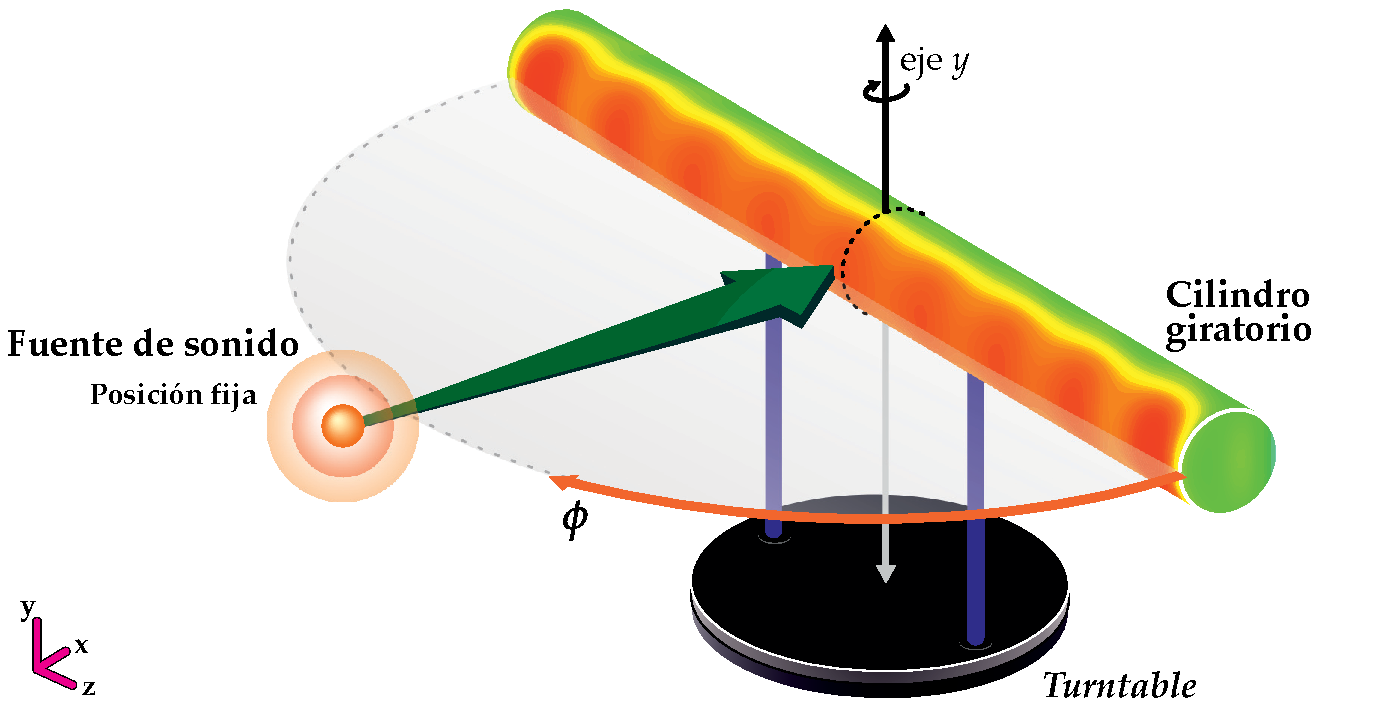
\includegraphics[width=0.72\linewidth]{figs/Measurement-Scheme-Fonseca-2013-sp.pdf}%
	\caption{Medición de \textit{beamforming} con arreglo cilíndrico (adaptado de Fonseca \cite{Fonseca-2013}) --- ejemplo de figura.}
	\label{fig:beamforming}%
\end{figure}


\begin{figure}[!ht]
  %\ContinuedFloat %% para continuar a partir de la figura anterior
  \centering
	\subfloat[Leyenda de la Figura~\protect\subref*{fig.figA}.]{\label{fig.figA}
            \makebox[.46\columnwidth]{\includegraphics[height=35mm,page=48]{example-image-duck}} } % makebox ayuda a organizar figs lado a lado
	\quad
  \subfloat[Leyenda de la Figura~\protect\subref*{fig.figB}.]{\label{fig.figB}
            \makebox[.46\columnwidth]{\includegraphics[height=35mm,page=47]{example-image-duck}} }
  \caption{Ejemplo de figuras lado a lado.}
  \label{subfig.exemplo}
\end{figure}


\begin{cuadro}[ht!] % En español
%\vspace{-2mm}
  \centering \ratb{1.3} \setlength\aboverulesep{0pt} \setlength\belowrulesep{0pt}
  \caption{Este es un ejemplo de un cuadro.}
    \fontsize{11}{12}\selectfont 
    \begin{tabular}{| C{2.8cm} | C{1.8cm} | C{1.8cm} |}
    \hline
	\SetRowColor{LightBlue}
    \textbf{ Experimento / Tipo } & \textbf{Exp. 1} & \textbf{Exp. 2}\\
	\midrule
		Tipo 1 & Verde & Amarilla\\
		\rowcolor[gray]{.95} Tipo 2 & Azul & Blanco\\
	\hline
    \end{tabular}
    \label{quad.exemplo}%
    \vspace{2mm}
\end{cuadro}%


\begin{table}[!htb]
  \centering \ratb{1.3} 
  \caption{Propiedades microgeométricas y macroscópicas de las capas porosas CPA 1 y CAUQ-B\\ (extraído de Mareze \etal \cite{Mareze-2017}) --- ejemplo de tabla.}
	\fontsize{11}{12}\selectfont 
    \begin{tabular}{C{2.9cm} | C{1.5cm} | C{1.5cm} | C{1.5cm} | C{1.5cm} | C{1.5cm} | C{1.0cm}| C{1.0cm}}
    \toprule
		\SetRowColor{LightOrange}
    \textbf{ Muestra / Parámetro } & $L\txu{p}$ \qquad [$\upmu$\! m] & $L\txu{a}$ \qquad [$\upmu$\! m] & $D\txu{p}$ \qquad [$\upmu$\! m] & $D\txu{a}$ \qquad [$\upmu$\! m] & $\sigma$ [Ns/m\txup{4}] & {$\phi$\quad [--]} & $\alpha_{\infty}$ [--]\\
	  \midrule
		CPA 1 $\Rightarrow$  3,0\% &	1359,81 & 1492,51 & 2344,05 & 1425,67 &	5131 &	0,218 &	1,63\\
		\rowcolor[gray]{.95} CAUQ-B $\Rightarrow$ 4,5\%	& 1598,29 &	701,24 & 2126,46 & 895,34 &	54989 &	0,070 &	2,89\\
    \bottomrule
    \end{tabular}
    \label{tab.exemplo}%
\end{table}%


%% Modelo de figuras lado a lado usando minipage
%\begin{figure*}[b]
    %\centering
    %\begin{minipage}[t]{.48\textwidth}
        %\centering
        %
\includegraphics[width=1\linewidth,page=2]{FIA-logo.pdf}
        %\caption{Figura del lado izquierdo.}
        %\label{fig:ladoE}
    %\end{minipage}%
		%\quad
    %\begin{minipage}[t]{0.48\textwidth}
        %\centering
        %
\includegraphics[width=1\linewidth,page=2]{FIA-logo.pdf}
        %\caption{Figura del lado derecho.}
        %\label{fig:ladoD}
    %\end{minipage}
%\end{figure*}


\begin{matlabcode}[Ejemplo de un extracto de código (haciendo que Matlab escriba Latex).]{code.matlalatex}
  syms x
  f = taylor(log(1+x));
  latex(f)
\end{matlabcode}

Todos los elementos (figuras y gráficos, por ejemplo) pueden ser en color o en tonos de gris. Evite la utilización de elementos textuales de otros autores sin la debida citación (y/o autorización). Es esencial que las figuras que presenten texto estén en el mismo idioma del artículo. Evite citas indirectas como \textit{Google Imágenes}, por ejemplo, así como se recomienda evitar el uso de bases de conocimiento volátiles.

Las referencias cruzadas deben hacerse para todos los elementos, por ejemplo: Figura~\ref{fig:beamforming} y Tabla~\ref{tab.exemplo} (con solo la primera letra en mayúscula, evite que haya un salto de línea entre el rótulo y el número correspondiente). Si existe una subfigura, use Figura~\subref*{fig.figA}, por ejemplo.

%%%%%%%%%%%%%%%%%%%%%%%%%%%%%%%%%%%%%%%%%%%%%%%%%%%%%%%%%%%%%%%%%%%%%%%%%%%%%%%%%%%%%%%%%%%%%%%%%%%%%%%%%%%%%%%%%%%
\section{Tipos de artículo}

El evento aceptará \textbf{envíos originales} (es decir, aún no publicados) de investigaciones científicas y aplicaciones de ingeniería, arquitectura, audio, física, matemáticas, terapia del lenguaje y áreas (y subáreas) afines. Así, se sugieren los siguientes tipos de documentos:
%
\begin{itemize}[topsep=0ex] \itemsep=2pt
	\item \textbf{Artículos técnicos y aplicados} (\textit{Technical and applied papers}):
	presentan material original a partir de aplicaciones de técnicas conocidas y/o en desarrollo. Deben describir métodos aplicados que estén en conformidad con normativas y/o que presenten resultados relevantes. Es fundamental que estos artículos despierten el interés de investigadores y profesionales en el área propuesta.
	
	\item \textbf{Artículos científicos} (\textit{Scientific papers}): 
	incluyen material original (ideas, modelos, experimentos, etc.) inédito, que contribuye significativamente al avance del conocimiento científico en el tema abordado. El contenido debe establecer una conexión con el \textit{estado del arte} existente en la literatura publicada.

	\item \textbf{Artículos de revisión} (\textit{Review papers}):
	abordan el \textit{estado del arte} sobre el tema en cuestión, elucidando desde conceptos básicos hasta aspectos más complejos. Este tipo de envío debe ser exhaustivo en relación a la literatura existente, cubriendo ampliamente ideas, modelos, experimentos, etc., ya desarrollados, aunque discrepen de la visión del autor. Es crucial que el tema sea de interés para la comunidad científica.
\end{itemize}

\vspace{5pt}

Las áreas temáticas del evento incluyen:
%	
\begin{enumerate}[topsep=0ex] \itemsep=0.0pt
    \item Acústica Arquitectónica y de la Edificación
    \item Acústica Biomédica y Bioacústica
    \item Acústica Computacional
    \vspace{-0.25em}
    \begin{enumerate}[noitemsep,topsep=0ex] 
        \item Imágenes acústicas y acústica virtual/auralización
    \end{enumerate}    
    \item Acústica Estructural y Vibraciones
    \item Acústica Física y Ultrasonidos
    \vspace{-0.25em}
    \begin{enumerate}[noitemsep,topsep=0ex]
        \item Metamateriales estructurados para el control de ruido y vibraciones
    \end{enumerate}    
    \item Acústica Forense
    \item Acústica Musical
    \item Acústica Psicológica y Fisiológica
    \item Acústica Subacuática
    \item Audio Profesional y Electroacústica
    \item Educación en Acústica
    \item Paisajes Sonoros y Ecoacústica
    \item Procesado de Señales en Acústica
    \item Ruido Ambiental, Industrial y Ocupacional
\end{enumerate}


%%%%%%%%%%%%%%%%%%%%%%%%%%%%%%%%%%%%%%%%%%%%%%%%%%%%%%%%%%%%%%%%%%%%%%%%%%%%%%%%%%%%%%%%%%%%%%%%%%%%%%%%%%%%%%%%%%%
%%%%%%%%%%%%%%%%%%%%%%%%%%%%%%%%%%%%%%%%%%%%%%%%%%%%%%%%%%%%%%%%%%%%%%%%%%%%%%%%%%%%%%%%%%%%%%%%%%%%%%%%%%%%%%%%%%%
\section{Organización del trabajo}

El trabajo debe estar estructurado; por lo tanto, se sugieren los siguientes ítems:
%
\begin{itemize}[noitemsep,topsep=0ex] \itemsep=3pt
	\item Introducción: visión general sobre el tema con definición de los objetivos del trabajo, indicando su relevancia.
	\item Fundamentos: sobre todo en artículos científicos, la fundamentación teórica principal necesaria para la comprensión del texto debe ser presentada y referenciada.
	\item Desarrollo: cómo se realizó el trabajo, incluyendo detalles de teoría, materiales y métodos empleados.
	\item Resultados y discusiones: parciales o conclusivos, según la modalidad del trabajo, haciendo referencia a mediciones y cálculos estadísticos aplicados, si es el caso.
	\item Conclusiones (o Consideraciones finales): basarse en las discusiones y objetivos, presentando apuntes y consideraciones que finalizan el estudio/aplicación.
	\item Agradecimientos: opcional, cuando sea pertinente. En esta sección se admiten también declaraciones sobre financiamiento de investigación/proyecto.
	\item Referencias: presentar las referencias bibliográficas citadas en el texto.
\end{itemize}
%
No es necesario que existan secciones con estos nombres. La organización también depende del tipo de artículo.
Otros elementos post-textuales como apéndices son opcionales.


%%%%%%%%%%%%%%%%%%%%%%%%%%%%%%%%%%%%%%%%%%%%%%%%%%%%%%%%%%%%%%%%%%%%%%%%%%%%%%%%%%%%%%%%%%%%%%%%%%%%%%%%%%%%%%%%%%%
\subsection{Citas y referencias}

Para la confección de las referencias se debe utilizar la norma vigente. Las referencias deben ser \textbf{numeradas conforme al orden de aparición}, utilizando corchetes \cite{Gomes-2015}. Todas las referencias deben ser citadas en el texto. Las referencias \cite{Mareze-2017,Fonseca-2013,Brandao-2017,Gomes-2015,Oppenheim-2010,Muller-2001,Mareze-2019,aev:piccini2020} de este modelo de artículo son solo ilustrativas (para efecto de comprensión).

Al final del documento se debe incluir la sección de referencias. Las entradas en esta sección deben tener tipografía con tamaño 10~pt, espaciado simple y espaciado de párrafo de 6~pt. Esta plantilla de \LaTeX\xspace usa el paquete {\ttfamily natbib} para la organización de las referencias. Además, se recomienda la utilización de gestores de bases de datos bibliográficas como \href{http://www.jabref.org/}{JabRef}, \href{http://www.mendeley.com}{Mendeley} y \href{https://www.zotero.org/}{Zotero}. En especial para usuarios de Word, Mendeley tiene un \textit{plugin} para formatear e insertar las referencias en el documento .docx.

Dependiendo del contexto, el nombre del autor puede o no ser escrito, observe algunos ejemplos a continuación:
%
\begin{itemize}[noitemsep,topsep=0ex] \itemsep=4pt
	\item 	``... Mareze \etal \cite{Mareze-2019} trabajaron con absorción de materiales porosos...'', o 
	
	\item ``... para el estudio de acústica de salas \cite{Brandao-2017} se recomienda la lectura de un libro de texto...'', o
	\item ``... aplicando la Transformada de Fourier en las señales de entrada \cite{Oppenheim-2010}. '', o también
	\item ``... \txtcite{Fonseca-2013} demostró el cálculo de difracción para superficies cilíndricas~\cite{Fonseca-2013}.''
\end{itemize}
%
Todos los autores que figuran en las referencias deben estar citados en el texto.

En referencias con hasta tres autores, por ejemplo, Müller y Massarani \cite{Muller-2001}, ambos deben ser citados (cuando sean mencionados). En el caso de más de tres autores, por ejemplo, Gomes \etal \cite{Gomes-2015}, se debe citar solo el último nombre del primer autor seguido de la expresión ``\etal''. Además, al citar más de una referencia, utilice solo un corchete, vea algunos ejemplos a continuación:
%
\begin{itemize}[noitemsep,topsep=0ex] \itemsep=8pt
	\item ``Trabajos en temas de acústica y vibraciones \cite{Mareze-2017,Fonseca-2013,Brandao-2017}.''
	\item ``Trabajos en temas de acústica \cite{Mareze-2017,Oppenheim-2010,Muller-2001, Mareze-2019, jasa:2022eac}.''
	%\item ``Trabajos con análisis estadístico \cite{Mareze-2017, Brandao-2017, aev:piccini2020}.''
	\item \textbf{No usar este estilo:} ``Trabajos con análisis estadístico \cite{Mareze-2017}, \cite{Brandao-2017}, \cite{jasa:2022eac} o \cite{Mareze-2017}--\cite{jasa:2022eac}.''
\end{itemize}
%
Se recomienda que las referencias sean ordenadas y compactadas (con guion) como en \cite{Mareze-2017,Oppenheim-2010,Muller-2001,Mareze-2019}.
%
En la sección de referencias, siempre que sea posible, incluya el ISBN, ISSN, DOI\footnote{Para usuarios de Latex basta usar el campo ``doi'' de su repositorio \texttt{.bib}.} (con enlace) y/o enlace con la dirección en línea donde el documento citado está disponible.

%%%%%%%%%%%%%%%%%%%%%%%%%%%%%%%%%%%%%%%%%%%%%%%%%%%%%%%%%%%%%%%%%%%%%%%%%%%%%%%%%%%%%%%%%%%%%%%%%%%%%%%%%%%%%%%%%%%
\section{Envío de artículos}

Los artículos completos deberán ser enviados por el sistema propio del congreso, disponible en el sitio web\linebreak \url{https://www.fia2024.cl}, dentro de los plazos establecidos. Detalles acerca del registro de autor participante pueden consultarse también en el sitio del evento o con la comisión organizadora.

Es responsabilidad de los autores la preparación y envío de los artículos en su formato final. Por este motivo, se pide que verifiquen con atención la formateo de sus artículos, especialmente gráficos y fotos, en cuanto a la legibilidad y calidad digital (y para impresión). \textbf{Los artículos deberán ser enviados en formato PDF (con tamaño máximo de 16~Mb).}

%Los metadatos del PDF para usuarios de \LaTeX\xspace se generan automáticamente, usuarios de MS Word deben verificar en el momento de la conversión.

%El uso de PDF-a es opcional.

%En investigaciones que involucren personas (o seres vivos en general), como en acústica subjetiva o fisiológica, por ejemplo, se recomienda aclarar en el artículo el término de aprobación del Comité de Ética, si es pertinente.


%%%%%%%%%%%%%%%%%%%%%%%%%%%%%%%%%%%%%%%%%%%%%%%%%%%%%%%%%%%%%%%%%%%%%%%%%%%%%%%%%%%%%%%%%%%%%%%%%%%%%%%%%%%%%%%%%%%
\subsection{Modelos para Word y \LaTeX}

El modelo de \LaTeX\xspace (\texttt{.tex}) fue escrito en codificación UTF8, por lo tanto, es compatible con Windows, Mac, Linux y \href{https://www.overleaf.com/read/tjbcfwbtfdtz\#869489}{Overleaf}\footnote{\url{https://www.overleaf.com/read/tjbcfwbtfdtz\#869489}.}. Puede ser usado libremente para la elaboración de los artículos.

El modelo de \texttt{.docx} fue creado en Microsoft Word 2016 y, con ello, sus funcionalidades de espaciado y configuraciones están garantizadas para esa versión. Todos ellos están disponibles con enlaces en el \href{https://www.fia2024.cl}{sitio del evento} (o \href{https://github.com/willdfonseca/latex}{en este repositorio}).

El autor de este texto y de los modelos es el profesor William D'Andrea Fonseca, de Ingeniería Acústica (EAC) de la Universidad Federal de Santa María (UFSM), Brasil.

%%%%%%%%%%%%%%%%%%%%%%%%%%%%%%%%%%%%%%%%%%%%%%%%%%%%%%%%%%%%%%%%%%%%%%%%%%%%%%%%%%%%%%%%%%%%%%%%%%%%%%%%%%%%%%%%%%%
\section{Consideraciones finales}

Este \textit{artículo modelo} tuvo como objetivo enumerar y esclarecer las directrices para el envío de trabajos al XIII~Congreso Iberoamericano de Acústica. Este documento sirve como una guía práctica, pudiendo ser utilizado como modelo al reemplazar su contenido según sea necesario.


%%%%%%%%%%%%%%%%%%%%%%%%%%%%%%%%%%%%%%%%%%%%%%%%%%%%%%%%%%%%%%%%%%%%%%%%%%%%%%%%%%%%%%%%%%%%%%%%%%%%%%%%%%%%%%%%%%%
\section{Agradecimientos}

Si es pertinente, haga agradecimientos.
%
En caso de trabajos con financiamiento, utilice esta sección para aclarar detalles.

%En el caso de este documento, nos gustaría agradecer la cooperación de todos para con el evento.

%%%%%%%%%%%%%%%%%%%%%%%%%%%%%%%%%%%%%%%%%%%%%%%%%%%%%%%%%%%%%%%%%%%%%%%%%%%%%%%%%%%%%%%%%%%%%%%%%%%%%%%%%%%%%%%%%%%
% EOF
